\chapter{Аналитическая часть}

\section{АВЛ-дерево}
АВЛ-дерево --- это один из видов бинарного дерева. Его особенностью заключается в том, что разница высот каждого поддерева не больше двух, такое дерево называется сбалансированным. Это позволяет гарантировать, что операции поиска и добавления элемента будут выполнены за логарифмическое время $O(log \ n)$, где $n$ --- высота дерева.

\section{Балансировка дерева}
\subsection{Малое левое вращение}
Малое левое вращение выполняется, когда разница высот между правым ($b$) и левым ($L$) поддеревом узла ($a$) равна 2, и высота левого поддерева узла $b$ ($C$) меньше либо равна высоте его правого поддерева ($R$). Для восстановления баланса узел $b$ становится новым корнем, узел $a$ перемещается в левое поддерево $b$, а поддерево $C$ становится правым поддеревом $a$. После вращения необходимо обновить высоты поддеревьев следующим образом: высота $a$ становится $max (height(L), height(C)) + 1$, а высота $b$ --- $max (height(a), height(R)) + 1$. После вращения баланс поддерева восстанавливается. На рисунке \ref{fig:2} изображено графическое пояснение малого левого вращения.
\begin{center}
	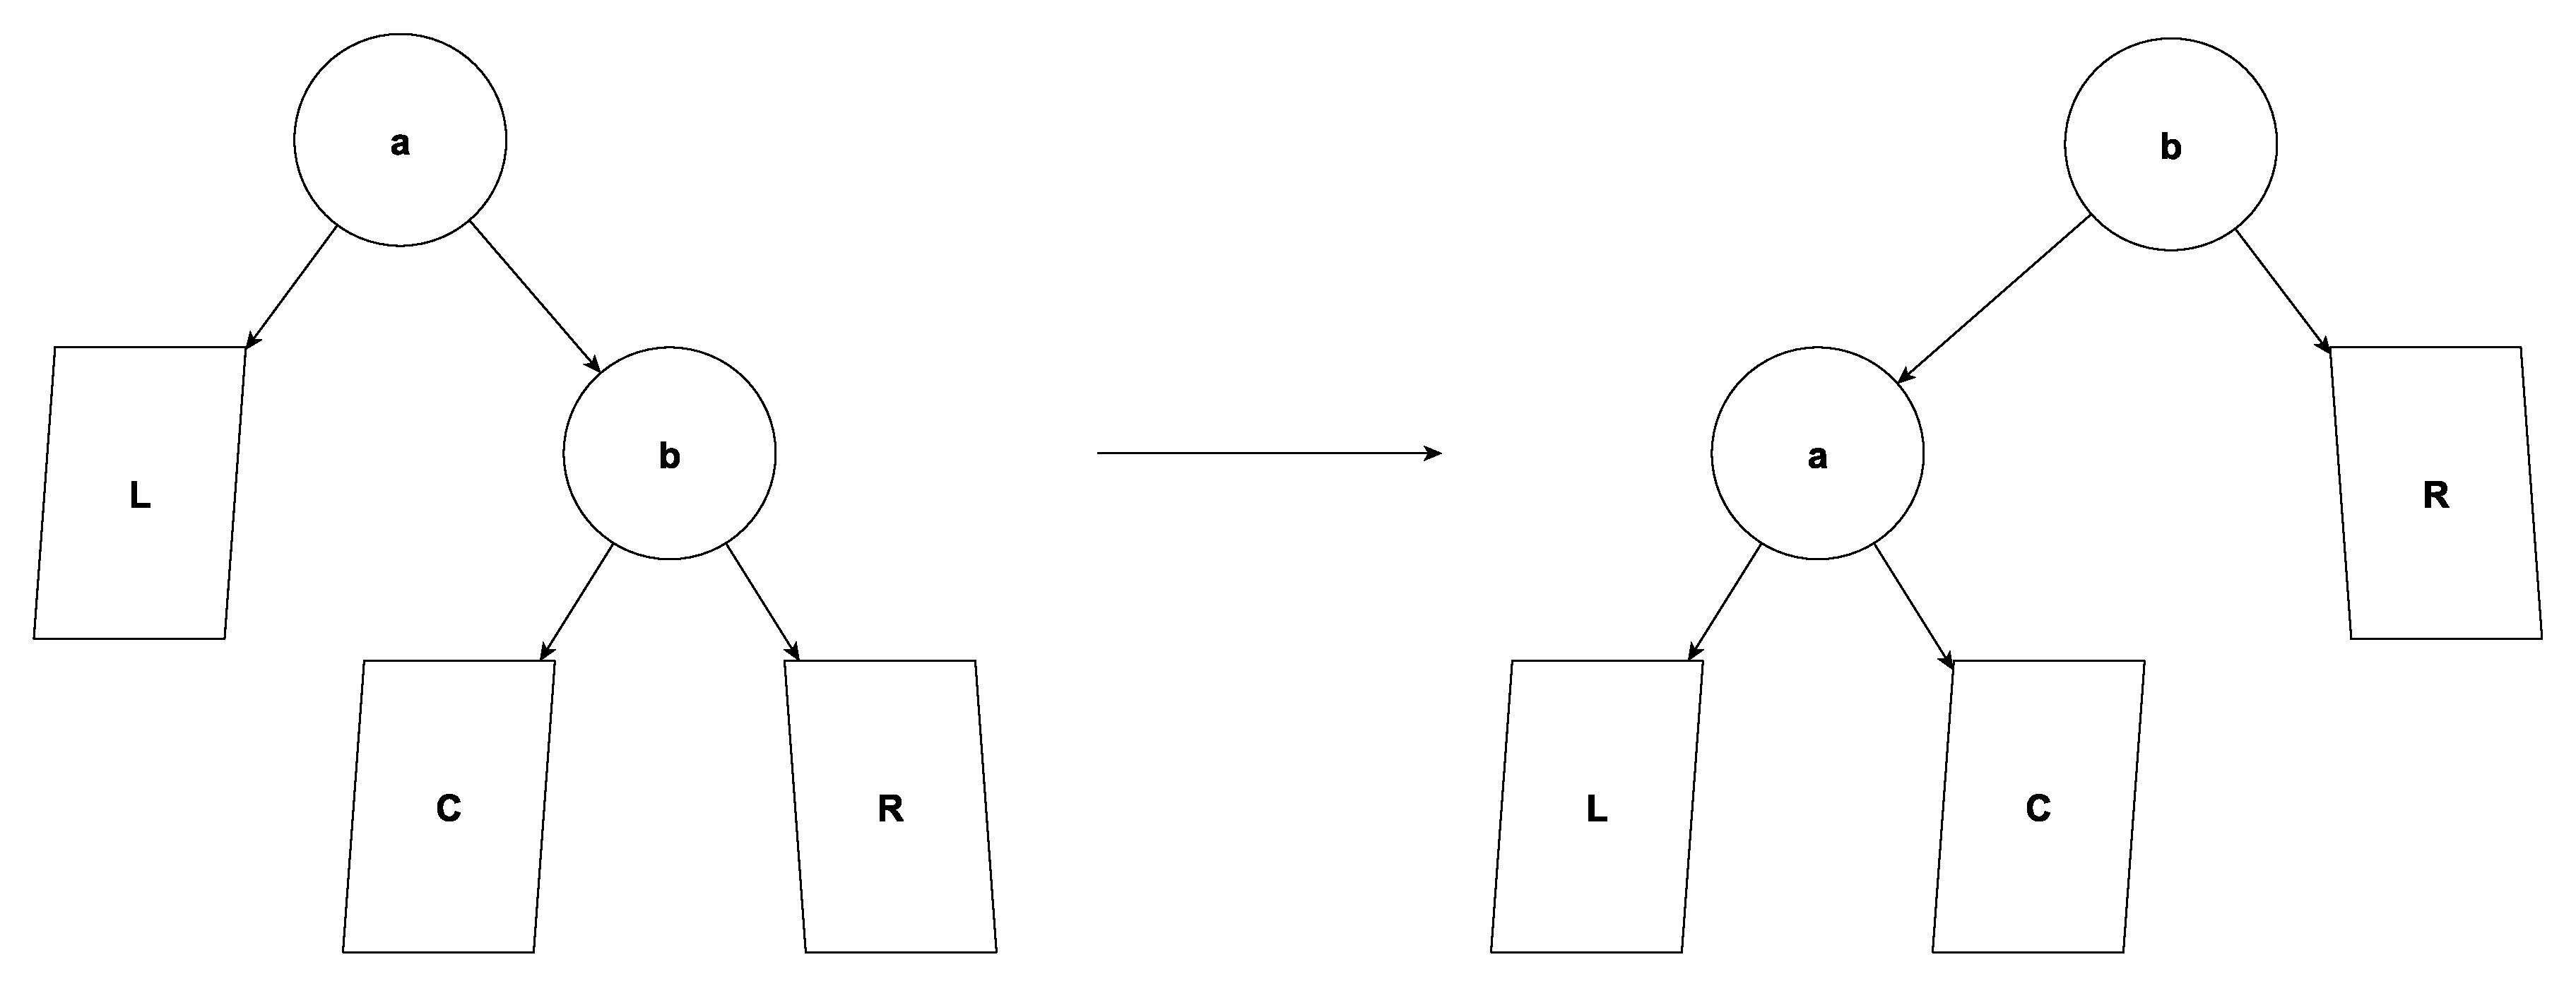
\includegraphics[scale = 0.2]{smallleft.eps}
	\captionof{figure}{Малое левое вращение}
	\label{fig:2}
\end{center}


\subsection{Малое правое вращение}
Малое правое вращение  выполняется, когда разница высот между правым ($b$) и левым ($L$) поддеревом узла ($a$) равна 2, и высота правого поддерева узла $b$ ($C$) меньше либо равна высоте его левого поддерева ($R$). Для восстановления баланса узел $b$ становится новым корнем, узел $a$ перемещается в правое поддерево $b$, а поддерево $C$ становится левым поддеревом $a$.После вращения необходимо обновить высоты поддеревьев следующим образом: высота $a$ становится $max (height(C), height(R)) + 1$, а высота $b$ --- $max (height(a), height(L)) + 1$. После вращения баланс поддерева восстанавливается. На рисунке \ref{fig:3} изображено графическое пояснение малого правого вращения.
\begin{center}
	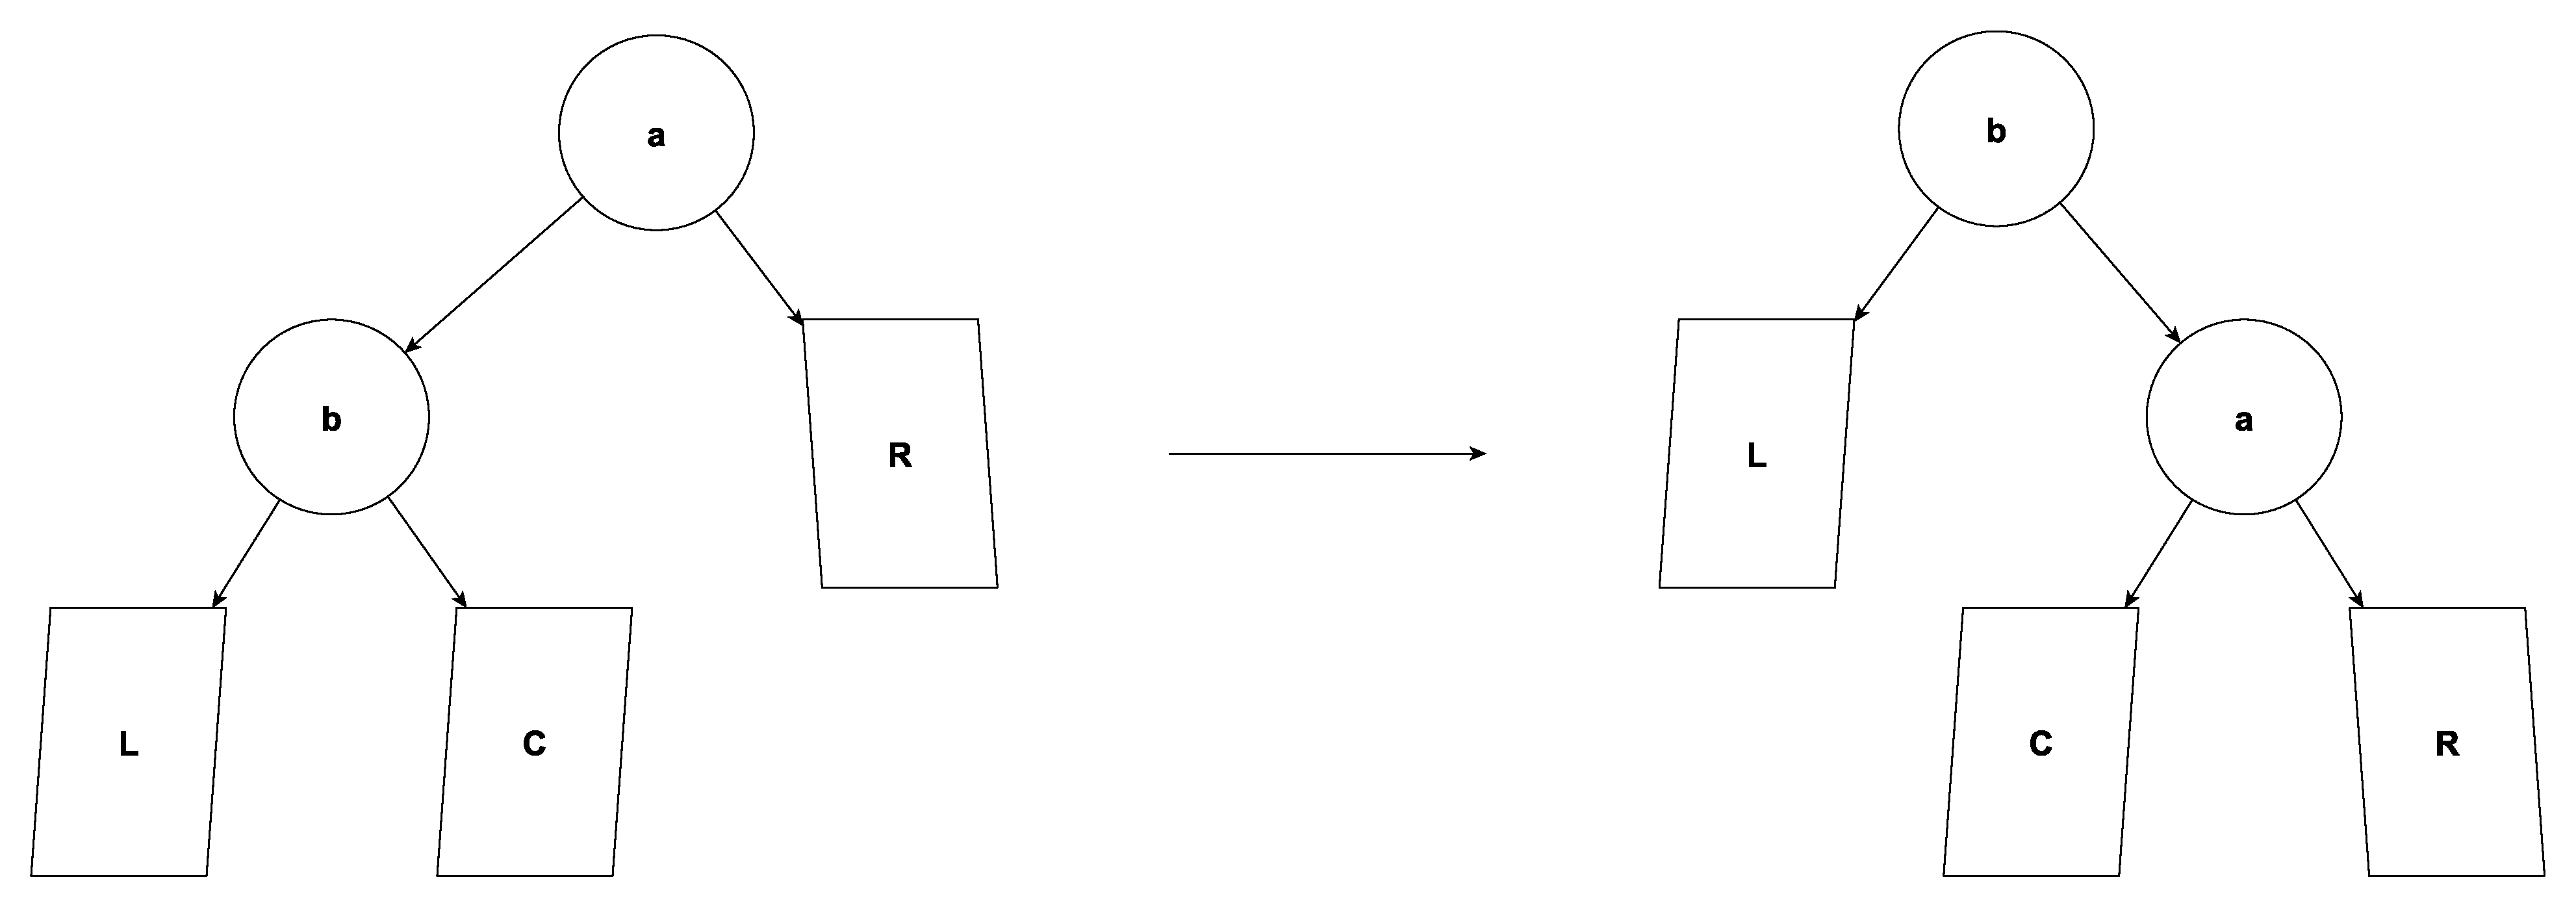
\includegraphics[scale = 0.2]{smallright.eps}
	\captionof{figure}{Малое правое вращение}
	\label{fig:3}
\end{center}

\subsection{Большое левое вращение}
Большое левое вращение выполняется, когда разница высот между правым ($b$) и левым ($L$) поддеревом узла ($a$) равна 2, а высота левого поддерева узла $b$ ($c$) больше высоты его правого поддерева ($R$). Для восстановления баланса сначала выполняется малое правое вращение относительно узла $b$: узел $c$ становится корнем правого поддерева узла $a$, узел $b$ перемещается в правое поддерево $c$, а поддерево $N$ становится левым поддеревом $b$. Затем выполняется малое левое вращение относительно узла $a$: узел $c$ становится новым корнем текущего поддерева, узел $a$ перемещается в левое поддерево $c$, а узел $b$ остаётся правым поддеревом $c$. Поддеревья $M$ и $N$ распределяются соответственно. Высоты узлов $a$, $b$ и $c$ пересчитываются, восстанавливая баланс. На рисунке \ref{fig:4} изображено графическое пояснение большого левого вращения. \newpage
\begin{center}
	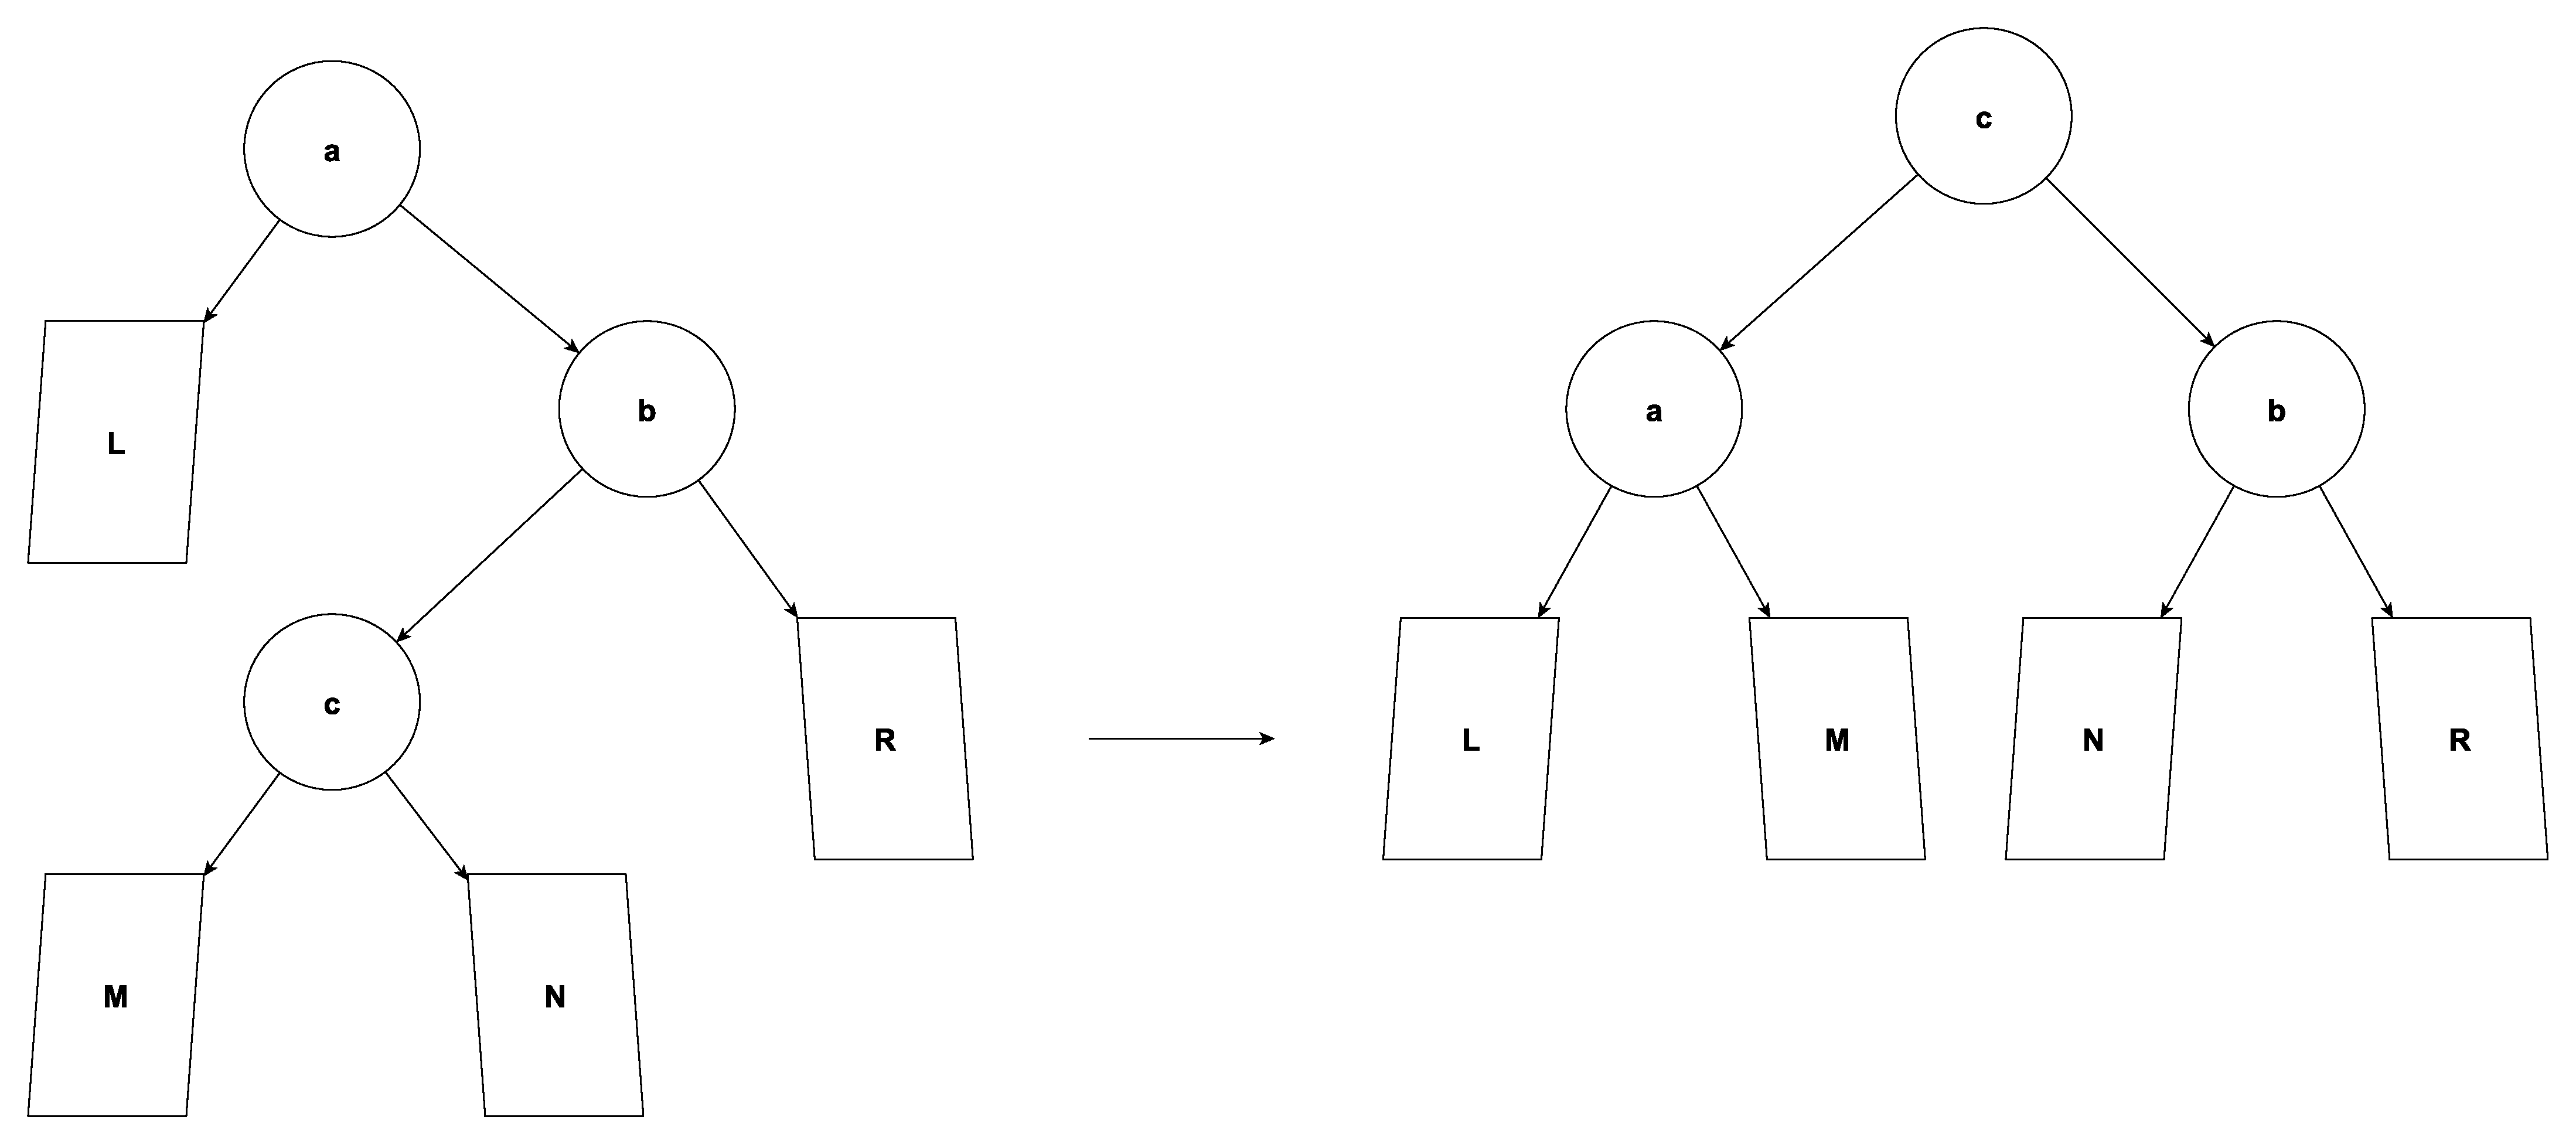
\includegraphics[scale = 0.2]{bigleft.eps}
	\captionof{figure}{Большое левое вращение}
	\label{fig:4}
\end{center}

\subsection{Большое правое вращение}
Большое правое вращение выполняется, когда разница высот между левым ($b$) и правым ($R$) поддеревом узла ($a$) равна 2, а высота правого поддерева узла $b$ ($c$) больше высоты его левого поддерева ($L$). Для восстановления баланса сначала выполняется малое левое вращение относительно узла $b$: узел $c$ становится корнем левого поддерева узла $a$, узел $b$ перемещается в левое поддерево $c$, а поддерево $M$ становится правым поддеревом $b$. Затем выполняется малое правое вращение относительно узла $a$: узел $c$ становится новым корнем текущего поддерева, узел $a$ перемещается в правое поддерево $c$, а узел $b$ остаётся левым поддеревом $c$. Поддеревья $L$ и $N$ распределяются соответственно. Высоты узлов $a$, $b$ и $c$ пересчитываются, восстанавливая баланс.
На рисунке \ref{fig:5} изображено графическое пояснение большого правого вращения.
\begin{center}
	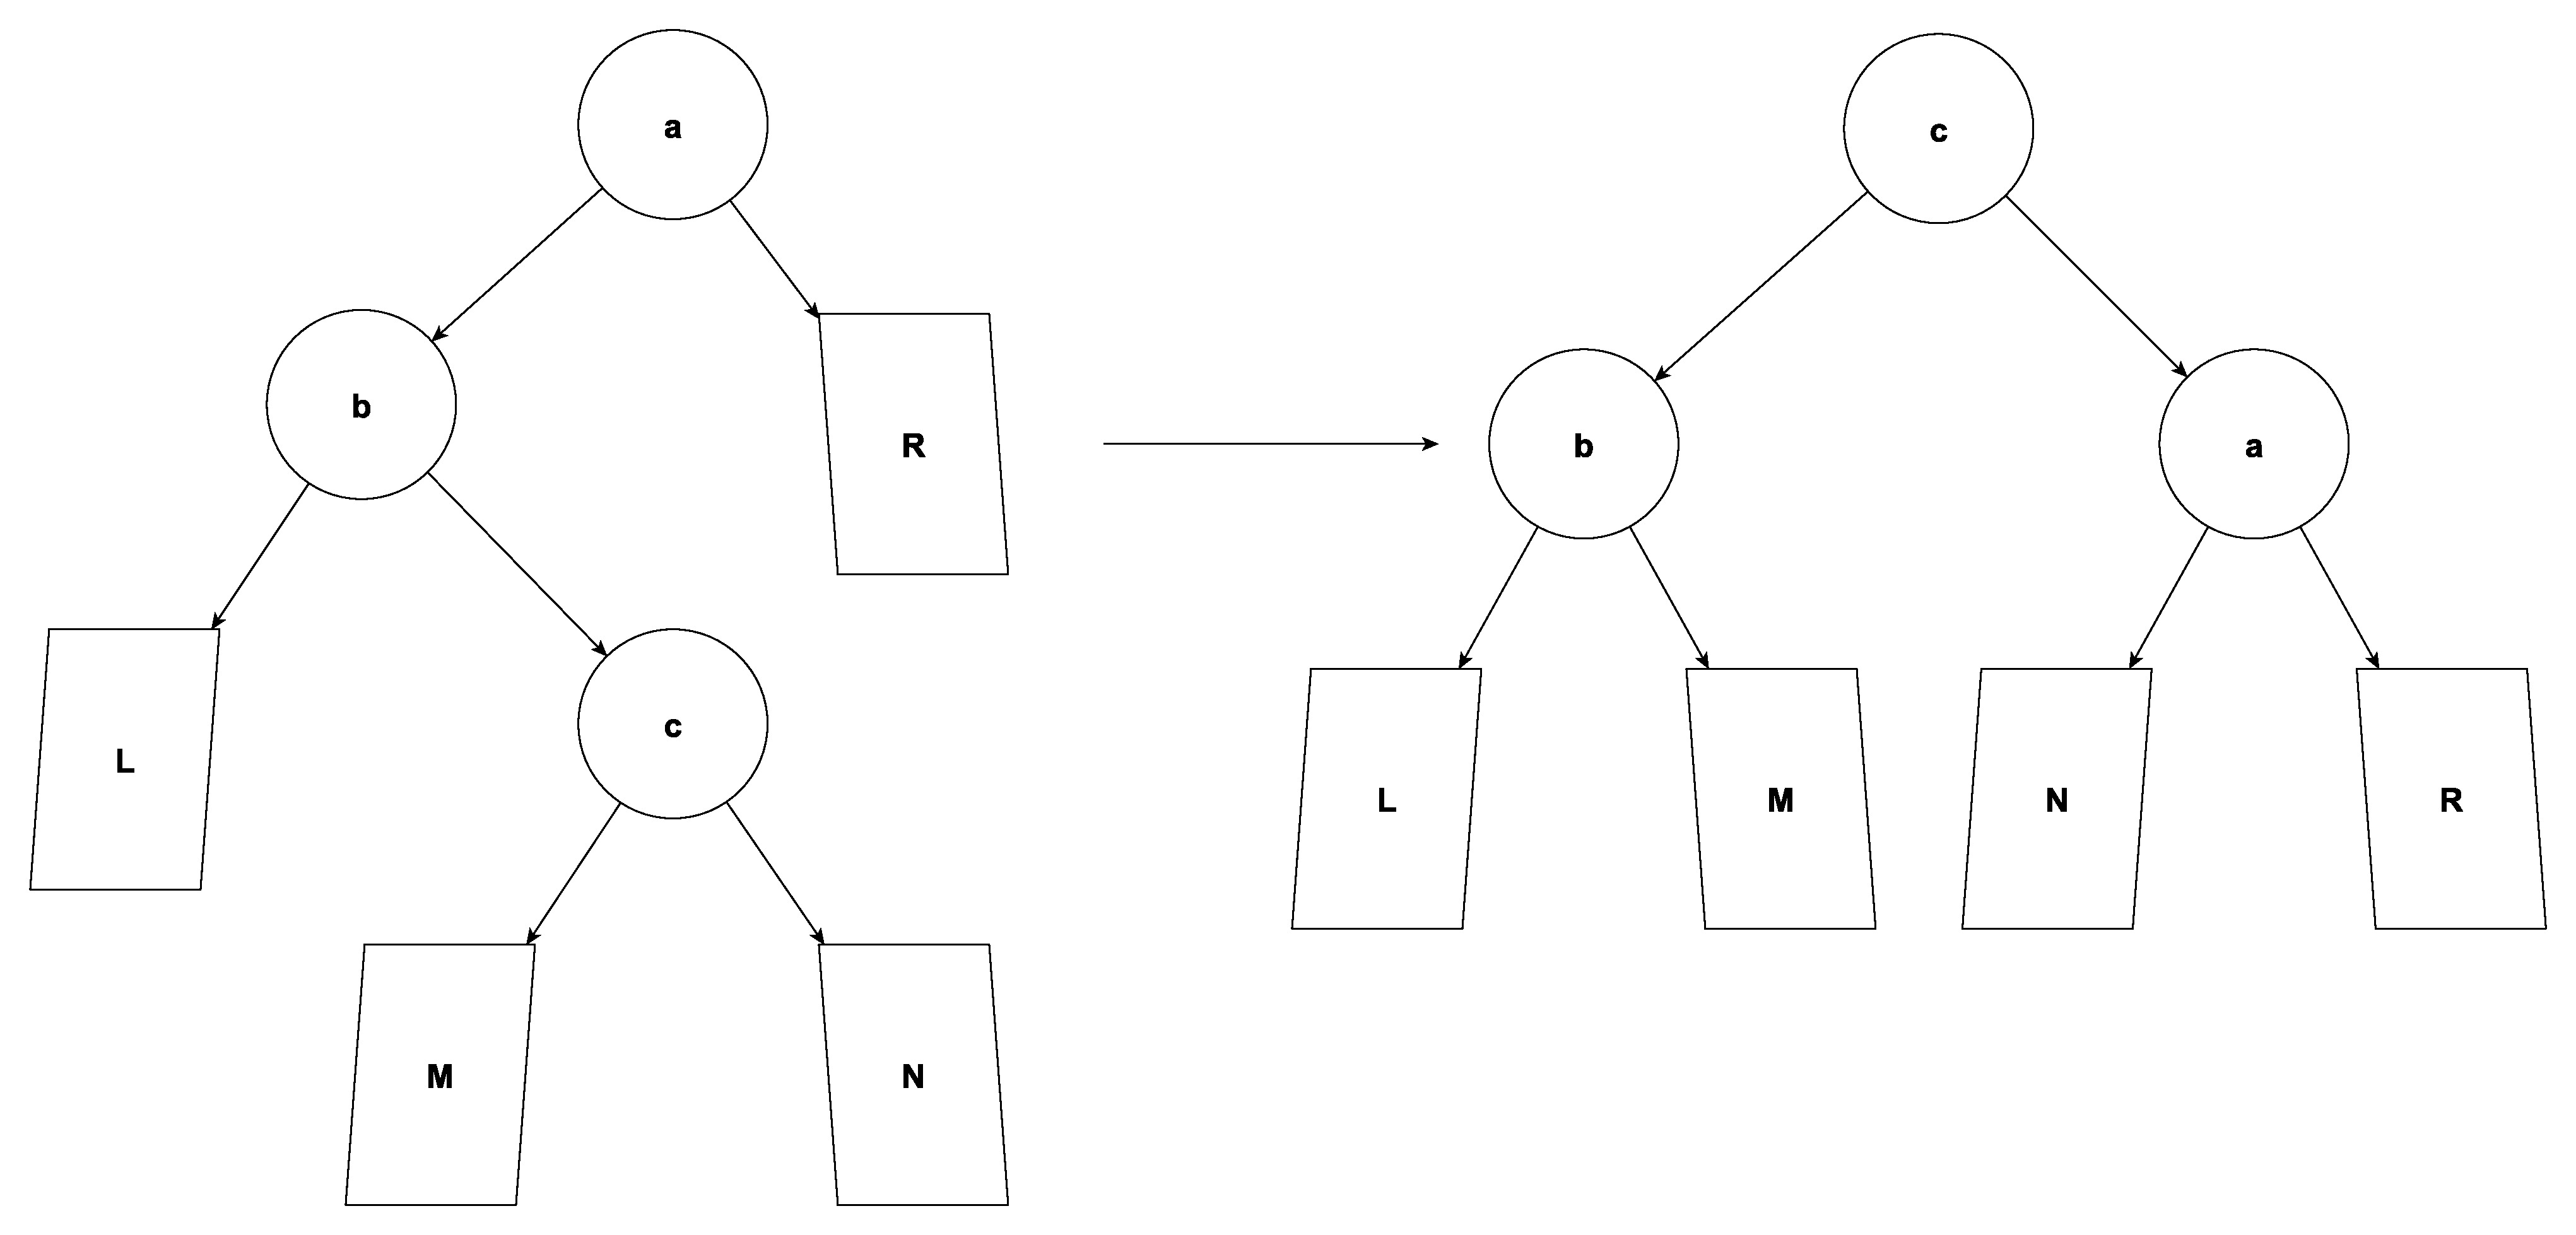
\includegraphics[scale = 0.2]{bigright.eps}
	\captionof{figure}{Большое правое вращение}
	\label{fig:5}
\end{center}
\clearpage
